\section{Angular Frontend}
\setauthor{Benjamin Ecker}

\subsection{Ordnerstruktur}
\begin{figure}[H]
    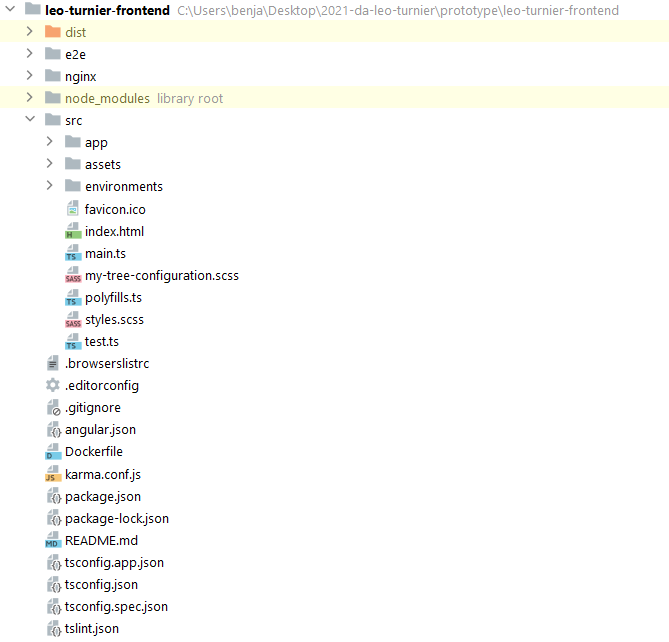
\includegraphics[scale=0.8]{pics/frontend/angular_file_structure.PNG}
    \caption{Angular Ordnerstruktur}
\end{figure}

Bei der Erstellung einer Angular Applikation wird schon fast die gesamte Ordnerstruktur festgelegt. Bis auf ein paar Ausnahmen wie der Nginx Ordner, oder die zwei in Gelb markierten Ordner,
welche nach dem dem Laden bzw. Builden generiert werden, hat sich hier nichts getan.
Wie an den meisten Filenamen schon zu erkennen ist befinden sich auf dieser Ebene so fast nur Files, die zur Konfiguration nötig sind. Das wichtigste File dabei ist "package.json".

\begin{figure}[H]
    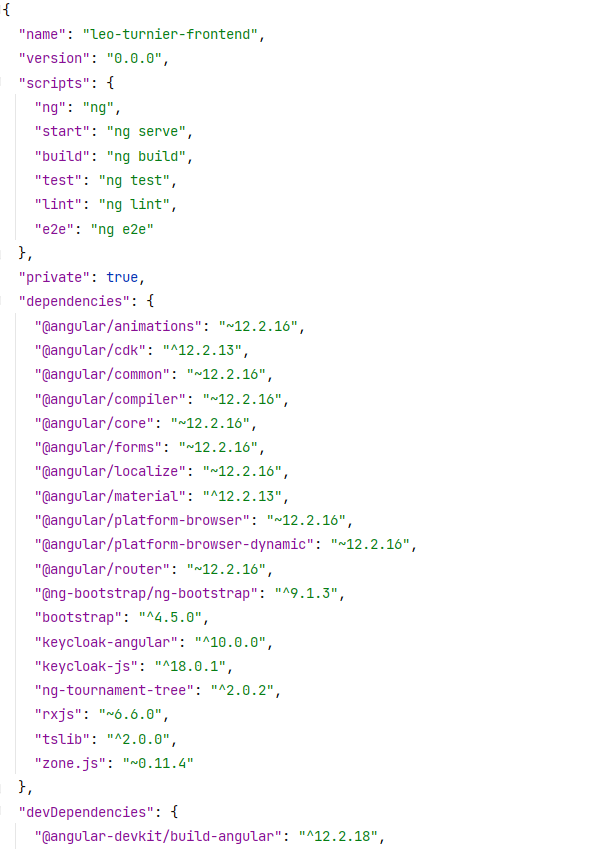
\includegraphics[scale=0.6]{pics/frontend/package_json.PNG}
    \caption{package.json}
\end{figure}

Hier werden alle Metadaten, Scripts und Dependencies der App aufgelistet.
Bei den Dependencies unterscheidet man zwischen Dependencies und DevDependencies.
\begin{itemize}
    \item Dependencies werden transitiv installiert: Wenn A B benötigt und B C benötigt, wird C installiert, sonst könnte B nicht funktionieren und A auch nicht.
    \item DevDependencies wird nicht transitiv installiert. Wir brauchen z.B. B nicht zu testen, um A zu testen, also können die Testabhängigkeiten von B weggelassen werden.
\end{itemize}

Um diese Dependencies auch nützen zu können muss bei jedem Angular Projekt "npm install" ausgeführt werden um diese zu Laden.
Danach werden sie dann im Ordner node\_modules gespeichert.
Dieser sollte, aber vor jeder Weitergabe gelöscht werden,oder wie zum Beispiel in Git im ".gitignore" inkludiert werden, da dieser mit Abstand am speicherintensivsten ist. 

\newpage
Auch wenn Angular eine große Anzahl an Ordnern und Files bietet geschieht wahrscheinlich 99\% der Arbeit eines Angular-Projekt im app Ordner.
Dieser enthält alle Components sowie Klassen die für die Applikation benötigt werden.

\begin{figure}[H]
    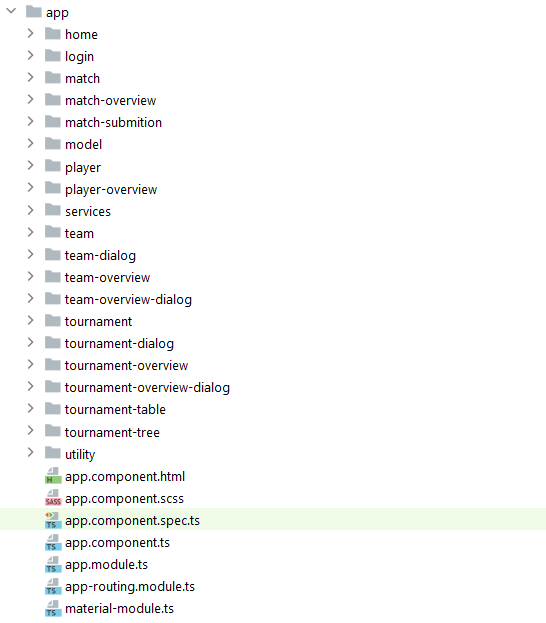
\includegraphics[scale=0.6]{pics/frontend/app_folder.PNG}
    \caption{App Ordner}
\end{figure}

Um ein bisschen Ordnung ins Chaos zu bringen kann man diese Files bzw Ordner in drei Kategorien unterteilen:
\begin{itemize}
    \item App Components: Alle Files die mit app anfangen
    \item Hilfklassen: model, services, utility, material-module.ts
    \item Components: Alle restlichen Ordner.
\end{itemize}

\subsection{App Components}